% Chapter: 01_theory
% Included from lectures/steganography/main.tex

\section{Steganography: Theory}

\begin{frame}{What is Steganography?}
\begin{columns}[T]
\begin{column}{0.47\textwidth}
\textbf{Cryptography}
\begin{itemize}
\item Hides the \textbf{content} of a message
\item Outsiders cannot read it
\item But everyone sees that a secret is being sent
\end{itemize}
\end{column}
\begin{column}{0.47\textwidth}
\textbf{Steganography}
\begin{itemize}
\item Hides the \textbf{existence} of a message
\item The secret sits inside an innocent-looking cover
\item An observer sees only ordinary communication
\end{itemize}
\end{column}
\end{columns}
\vspace{1.5em}
\begin{center}
Covers can be images, text, sound files or even network protocols.
\end{center}

\note{
\begin{itemize}
\item Steganography is the art and science of hidden communication
\item Cryptography protects the content of a message by making it unreadable to outsiders
\item Steganography conceals the very existence of the message
\item The secret is embedded in an innocent-looking cover: an image, a line of text, a sound file, a network protocol
\item Core question: how can information be transmitted without revealing that communication is taking place at all?
\item Link back to the Stego Game from this morning
\end{itemize}
}
\end{frame}

\begin{frame}{The Setup}
\begin{center}
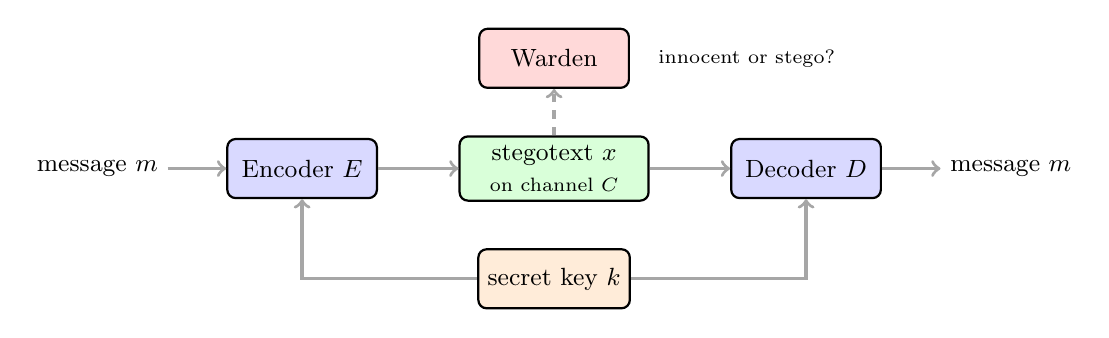
\begin{tikzpicture}[
  box/.style={rectangle, draw, thick, rounded corners=3pt, minimum width=1.9cm, minimum height=0.75cm, font=\small},
  arr/.style={->, very thick, gray!70},
]
  \node[font=\small] (m) at (0, 0) {message $m$};
  \node[box, fill=blue!15] (enc) at (2.6, 0) {Encoder $E$};
  \node[box, fill=green!15, minimum width=2.4cm, align=center] (x) at (5.8, 0) {stegotext $x$ \\ {\scriptsize on channel $C$}};
  \node[box, fill=blue!15] (dec) at (9.0, 0) {Decoder $D$};
  \node[font=\small] (m2) at (11.6, 0) {message $m$};
  \node[box, fill=orange!15] (key) at (5.8, -1.4) {secret key $k$};
  \node[box, fill=red!15] (w) at (5.8, 1.4) {Warden};

  \draw[arr] (m) -- (enc);
  \draw[arr] (enc) -- (x);
  \draw[arr] (x) -- (dec);
  \draw[arr] (dec) -- (m2);
  \draw[arr] (key) -| (enc);
  \draw[arr] (key) -| (dec);
  \draw[arr, dashed] (x) -- (w);
  \node[font=\scriptsize, right] at (7.0, 1.4) {innocent or stego?};
\end{tikzpicture}
\end{center}
\vspace{-0.5em}
\begin{columns}[T]
\begin{column}{0.47\textwidth}
\small
\begin{itemize}
\item Encoder $E$ and decoder $D$ share a secret key $k$
\item A channel $C$ carries the messages
\item A distribution $\mathcal{D}$ of innocent messages
\item A message space $M$ of possible secrets
\end{itemize}
\end{column}
\begin{column}{0.47\textwidth}
\small
\begin{itemize}
\item A warden observes the channel
\item \textbf{Correctness}: decoding succeeds with high probability
\item \textbf{Security}: the warden's distinguishing advantage is small
\end{itemize}
\end{column}
\end{columns}

\note{
\begin{itemize}
\item Sender and receiver are often called encoder and decoder, they share a secret key
\item The channel is where messages are transmitted
\item The innocent distribution describes what ordinary communication over the channel looks like
\item The message space contains the secret messages the sender may wish to transmit
\item The encoding procedure embeds a secret message into an apparently innocent message
\item The decoding procedure recovers it
\item The adversary, or warden, observes the communication and tries to distinguish ordinary messages from steganographic ones
\item Two conditions: correctness and security
\item Ask: who played which role in the Stego Game?
\end{itemize}
}
\end{frame}

\begin{frame}{Detection as Hypothesis Testing}
\begin{columns}[c]
\begin{column}{0.5\textwidth}
\begin{description}
\item[Innocent channel] the normal language model
\item[Covertext] the model's response
\item[Hidden message] a payload embedded in the response
\item[Adversary] sees the response and decides: ordinary or stego?
\end{description}
\end{column}
\begin{column}{0.45\textwidth}
For a prompt $p$:
\begin{align*}
P &= \mathrm{Model}(p) && \text{innocent} \\
Q &= \mathrm{Steg}_k(p, m) && \text{stego}
\end{align*}
The adversary tests
\begin{align*}
H_0 &: x \sim P \\
H_1 &: x \sim Q
\end{align*}
\end{column}
\end{columns}

\note{
\begin{itemize}
\item Now the same setup in the LLM setting
\item The innocent channel is the normal language model, the covertext is the model's response
\item The hidden message is a payload embedded in that response
\item $P$ is the innocent distribution over responses for a prompt $p$
\item $Q$ is the steganographic distribution when hiding message $m$ with key $k$
\item The adversary performs hypothesis testing between the two
\item The goal is that the adversary cannot reliably distinguish these two cases
\end{itemize}
}
\end{frame}

\begin{frame}{Perfect Security}
The strongest notion is \textbf{perfect information-theoretic indistinguishability}:
$$P = Q \quad \Longleftrightarrow \quad d_{\mathrm{TV}}(P, Q) = 0$$
with the total variation distance
$$d_{\mathrm{TV}}(P, Q) = \frac{1}{2} \sum_x |P(x) - Q(x)|$$
\vspace{0.5em}
\begin{itemize}
\item One sample, equal priors: the best possible adversary succeeds with probability
$$\Pr[\text{correct}] = \frac{1}{2}\left(1 + d_{\mathrm{TV}}(P, Q)\right)$$
\item If $d_{\mathrm{TV}} = 0$, no adversary can do better than guessing, even with unlimited computation
\end{itemize}

\note{
\begin{itemize}
\item Perfect security means the stego output distribution is exactly the same as the innocent output distribution
\item Total variation distance is the operational distance for hypothesis testing
\item If the adversary gets one sample and both hypotheses have equal prior probability, the optimal success probability is $\frac{1}{2}(1 + d_{\mathrm{TV}})$
\item So with $d_{\mathrm{TV}} = 0$ no adversary, even an unbounded one, can distinguish stego output from innocent output
\item Question for the room: can we have this? What does it cost?
\end{itemize}
}
\end{frame}

\begin{frame}{Perfect Security Needs Long Keys}
\begin{columns}[c]
\begin{column}{0.54\textwidth}
$M$: message, $X$: stegotext, $K$: key
\begin{itemize}
\item Perfect security: $I(M; X) = 0$
\item Perfect decoding: $H(M \mid X, K) = 0$
\end{itemize}
\vspace{0.5em}
\small
\begin{align*}
H(M) &= H(M \mid X, K) + I(M; X, K) \\
     &= \underbrace{H(M \mid X, K)}_{=0} + \underbrace{I(M; X)}_{=0} + I(M; K \mid X) \\
     &\leq H(K \mid X) \leq H(K)
\end{align*}
\end{column}
\begin{column}{0.44\textwidth}
\begin{center}
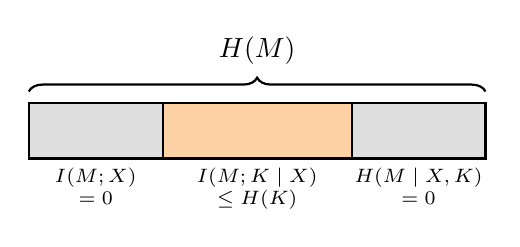
\begin{tikzpicture}
  \fill[gray!25] (0, 0) rectangle (1.7, 0.7);
  \fill[orange!35] (1.7, 0) rectangle (4.1, 0.7);
  \fill[gray!25] (4.1, 0) rectangle (5.8, 0.7);
  \draw[thick] (0, 0) rectangle (5.8, 0.7);
  \draw[thick] (1.7, 0) -- (1.7, 0.7);
  \draw[thick] (4.1, 0) -- (4.1, 0.7);
  \draw[decorate, decoration={brace, amplitude=5pt}, thick] (0, 0.85) -- (5.8, 0.85)
    node[midway, above=6pt] {$H(M)$};
  \node[below, font=\scriptsize, align=center] at (0.85, 0) {$I(M; X)$ \\ $= 0$};
  \node[below, font=\scriptsize, align=center] at (2.9, 0) {$I(M; K \mid X)$ \\ $\leq H(K)$};
  \node[below, font=\scriptsize, align=center] at (4.95, 0) {$H(M \mid X, K)$ \\ $= 0$};
\end{tikzpicture}
\end{center}
\vspace{1em}
\begin{center}
\fbox{$H(M) \leq H(K)$}
\end{center}
\end{column}
\end{columns}

\note{
\begin{itemize}
\item Perfect hiddenness: the observed stegotext reveals no information about the hidden message
\item Perfect decoding: the receiver recovers $M$ exactly from the stegotext and the key
\item First line is the definition of mutual information, second line is the chain rule
\item Mutual information is bounded by entropy: $I(M; K \mid X) \leq H(K \mid X) \leq H(K)$
\item The picture: the entropy of the message splits into three parts, two of them are forced to zero
\item Result: the shared secret must contain at least as much entropy as the hidden message
\end{itemize}
}
\end{frame}

\begin{frame}{Why This Is Impractical}
\begin{itemize}
\item The key has to grow linearly with the message
\item Arbitrarily many hidden messages need an unbounded supply of shared randomness, or a way to refresh it
\item This is the one-time pad again: perfect secrecy consumes key material
\item Whoever can exchange that much secret randomness could often use that channel directly
\end{itemize}
\vspace{1em}
Steganography is still not useless: it hides the \textbf{existence} of communication, encryption only hides the \textbf{content}.

\vspace{1em}
Practical schemes use a short reusable key and settle for \textbf{computational security}.

\note{
\begin{itemize}
\item $H(M) \leq H(K)$ means the key length scales linearly with the message length
\item A finite fixed key is not enough for arbitrarily many hidden messages
\item Analogous to the one-time pad
\item If sender and receiver already have a secret channel for large amounts of fresh randomness, they could often use it directly for communication or key refreshment
\item That does not make steganography useless, since it hides the existence of communication
\item But perfect information-theoretic steganography is usually expensive in secret randomness
\item So practical schemes use a short reusable key
\end{itemize}
}
\end{frame}

\begin{frame}{Computational Security}
Weaken the requirement:
\vspace{0.5em}
\begin{columns}[T]
\begin{column}{0.47\textwidth}
\textbf{Perfect}
\begin{itemize}
\item $P = Q$
\item \emph{No one} can distinguish the two distributions
\end{itemize}
\end{column}
\begin{column}{0.47\textwidth}
\textbf{Computational}
\begin{itemize}
\item $P \approx Q$ for efficient observers
\item No \emph{polynomial-time} adversary can distinguish them with non-negligible advantage
\end{itemize}
\end{column}
\end{columns}
\vspace{1.5em}
\begin{center}
An unbounded adversary may still break the scheme.
\end{center}

\note{
\begin{itemize}
\item Instead of demanding $P = Q$ against all adversaries, we demand that no efficient adversary can distinguish $P$ from $Q$
\item The guarantee is not: no one can distinguish the two distributions
\item It is: no polynomial-time adversary can distinguish them with non-negligible advantage
\item This is a reasonable assumption about real adversaries
\item An unbounded adversary may still break the scheme
\end{itemize}
}
\end{frame}

\begin{frame}{Pseudorandom Functions}
A \textbf{PRF} is a family of keyed functions
$$F = \left\{ F_k : \{0,1\}^{\ell_1(\lambda)} \to \{0,1\}^{\ell_2(\lambda)} \;\middle|\; k \in \{0,1\}^{\lambda} \right\}$$
\begin{enumerate}
\item $F_k$ is efficiently computable given $k$
\item For every polynomial-time distinguisher $D$ and a truly random function $f$:
$$\left| \Pr_{k}\left[ D^{F_k}(1^\lambda) = 1 \right] - \Pr_{f}\left[ D^{f}(1^\lambda) = 1 \right] \right| \leq \mathrm{negl}(\lambda)$$
\end{enumerate}
\vspace{0.5em}
A short key, but to efficient algorithms it looks like a truly random function.

\note{
\begin{itemize}
\item $\lambda$ is the key length, input and output lengths are polynomial in $\lambda$
\item The distinguisher gets oracle access: it can query the function but does not see the key
\item $f$ is a truly random function with the same domain and range
\item Intuition: a truly random function requires an enormous amount of randomness
\item A PRF uses only a short key
\item But to efficient algorithms it looks like a truly random function
\end{itemize}
}
\end{frame}

\begin{frame}{Assumptions and Attack Cost}
\begin{columns}[T]
\begin{column}{0.47\textwidth}
\textbf{Assumption}
\begin{itemize}
\item One-way functions exist
\item This implies that PRFs exist
\item $P \neq NP$ alone is too weak for modern cryptography
\end{itemize}
\vspace{0.5em}
\textbf{Security argument}
\begin{enumerate}
\item Assume secure PRFs exist
\item Replace true randomness by PRF output
\item Efficient adversaries cannot tell the difference
\item So they cannot tell stego from innocent output
\end{enumerate}
\end{column}
\begin{column}{0.47\textwidth}
\textbf{Attack cost}
\begin{itemize}
\item Generic attack: try all keys of length $\lambda$
$$O(2^\lambda)$$
\item For each key, check whether the text has the expected statistical structure
\item A weak PRF or a flawed construction allows faster attacks
\item A good scheme makes exhaustive search the best strategy
\end{itemize}
\end{column}
\end{columns}

\note{
\begin{itemize}
\item The relevant assumption is not simply $P \neq NP$, that is too weak for modern cryptography
\item The standard assumption is the existence of one-way functions, which implies the existence of PRFs
\item Go through the four steps of the security argument
\item Efficient adversaries cannot distinguish stego output from innocent output, except with negligible advantage
\item Brute force: for each candidate key the attacker checks whether the observed text has the statistical structure expected under that key
\item If the correct key is found, the attacker can run the retrieval algorithm and decode the payload
\item The attack cost is at most $2^\lambda$ by exhaustive search
\item An unbounded adversary can still brute-force the key
\end{itemize}
}
\end{frame}

\begin{frame}{Summary: The Trade-off}
\begin{center}
\renewcommand{\arraystretch}{1.4}
\begin{tabular}{lll}
\toprule
 & \textbf{Perfect} & \textbf{Computational} \\
\midrule
Guarantee & $P_{\text{stego}} = P_{\text{innocent}}$ & no efficient distinguisher \\
Key & $H(K) \geq H(M)$, fresh & short, reusable \\
Assumption & none & secure PRFs exist \\
Unbounded adversary & still secure & breaks it, cost up to $2^\lambda$ \\
\bottomrule
\end{tabular}
\end{center}

\note{
\begin{itemize}
\item Perfect information-theoretic steganography requires the stego distribution to equal the innocent distribution exactly
\item With perfect decoding it requires $H(K) \geq H(M)$
\item So unlimited perfect hidden communication requires an unlimited or refreshed secret resource
\item Computational steganography uses a short reusable key and a PRF
\item The output is computationally indistinguishable from innocent model output, assuming the PRF is secure
\item Practical, but only against efficient adversaries
\end{itemize}
}
\end{frame}
